%%%%
\chapter{Sliding Window}

The Sliding Window pattern is used to perform a required operation on a specific window size of a given array or linked list, such as finding the longest subarray containing all 1s. Sliding Windows start from the 1st element and keep shifting right by one element and adjust the length of the window according to the problem that you are solving. In some cases, the window size remains constant and in other cases the sizes grows or shrinks.

\noindent
\\Following are some ways you can identify that the given problem might require a sliding window:

\begin{itemize}
    \item The problem input is a linear data structure such as a linked list, array, or string
    \item You’re asked to find the longest/shortest substring, subarray, or a desired value
\end{itemize}

\noindent
Common problems you use the sliding window pattern with:

\begin{itemize}
    \item Maximum sum subarray of size ‘K’ (easy)
    \item Longest substring with ‘K’ distinct characters (medium)
    \item String anagrams (hard)
\end{itemize}

\begin{figure}
	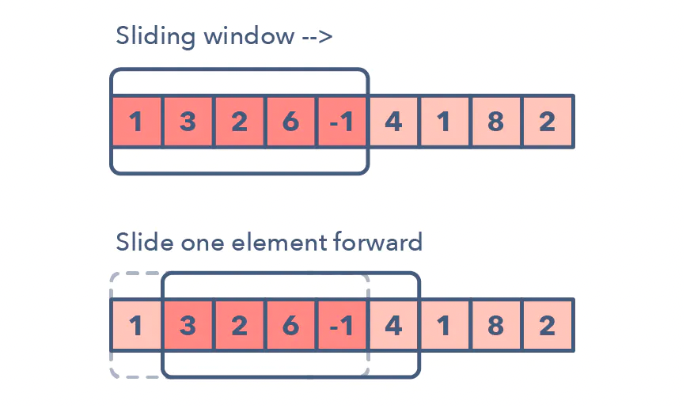
\includegraphics[width=0.45\linewidth]{slidingwindow}
\end{figure}



\section{Maximum Sum Subarray of Size K (easy)}

Problem Statement

\noindent
\\Given an array of characters where each character represents a fruit tree, you are given two baskets and your goal is to put maximum number of fruits in each basket. The only restriction is that each basket can have only one type of fruit.

\noindent
\\You can start with any tree, but once you have started you can’t skip a tree. You will pick one fruit from each tree until you cannot, i.e., you will stop when you have to pick from a third fruit type.

\noindent
\\Write a function to return the maximum number of fruits in both the baskets.

Example 1:

Input: Fruit=['A', 'B', 'C', 'A', 'C']

Output: 3

Explanation: We can put 2 'C' in one basket and one 'A' in the other from the subarray ['C', 'A', 'C']

Example 2:

Input: Fruit=['A', 'B', 'C', 'B', 'B', 'C']

Output: 5

Explanation: We can put 3 'B' in one basket and two 'C' in the other basket. 
This can be done if we start with the second letter: ['B', 'C', 'B', 'B', 'C']


answer

\lstset{language=Python}
\begin{lstlisting}

def fruits_into_baskets(fruits):
  window_start = 0
  max_length = 0
  fruit_frequency = {}

  # try to extend the range [window_start, window_end]
  for window_end in range(len(fruits)):
    right_fruit = fruits[window_end]
    if right_fruit not in fruit_frequency:
      fruit_frequency[right_fruit] = 0
    fruit_frequency[right_fruit] += 1

    # shrink the sliding window, until we are left with '2' fruits in 
    # the fruit frequency dictionary
    while len(fruit_frequency) > 2:
      left_fruit = fruits[window_start]
      fruit_frequency[left_fruit] -= 1
      if fruit_frequency[left_fruit] == 0:
        del fruit_frequency[left_fruit]
      window_start += 1  # shrink the window
    max_length = max(max_length, window_end-window_start + 1)
  return max_length


def main():
  print("Maximum number of fruits: " + 
  str(fruits_into_baskets(['A', 'B', 'C', 'A', 'C'])))
  print("Maximum number of fruits: " + 
  str(fruits_into_baskets(['A', 'B', 'C', 'B', 'B', 'C'])))

listing with colo
main()
    
\end{lstlisting}
\section{Fruits into Baskets (medium)}

Problem Statement

\noindent
\\Given an array of characters where each character represents a fruit tree, you are given two baskets and your goal is to put maximum number of fruits in each basket. The only restriction is that each basket can have only one type of fruit.

\noindent
\\You can start with any tree, but once you have started you can’t skip a tree. You will pick one fruit from each tree until you cannot, i.e., you will stop when you have to pick from a third fruit type.

\noindent
\\Write a function to return the maximum number of fruits in both the baskets.

Example 1:

Input: Fruit=['A', 'B', 'C', 'A', 'C']

Output: 3

Explanation: We can put 2 'C' in one basket and one 'A' in the other from the subarray ['C', 'A', 'C']

Example 2:

Input: Fruit=['A', 'B', 'C', 'B', 'B', 'C']

Output: 5

Explanation: We can put 3 'B' in one basket and two 'C' in the other basket. 
This can be done if we start with the second letter: ['B', 'C', 'B', 'B', 'C']


answer

\lstset{language=Python}
\begin{lstlisting}

def fruits_into_baskets(fruits):
  window_start = 0
  max_length = 0
  fruit_frequency = {}

  # try to extend the range [window_start, window_end]
  for window_end in range(len(fruits)):
    right_fruit = fruits[window_end]
    if right_fruit not in fruit_frequency:
      fruit_frequency[right_fruit] = 0
    fruit_frequency[right_fruit] += 1

    # shrink the sliding window, until we are left with '2' fruits in 
    # the fruit frequency dictionary
    while len(fruit_frequency) > 2:
      left_fruit = fruits[window_start]
      fruit_frequency[left_fruit] -= 1
      if fruit_frequency[left_fruit] == 0:
        del fruit_frequency[left_fruit]
      window_start += 1  # shrink the window
    max_length = max(max_length, window_end-window_start + 1)
  return max_length


def main():
  print("Maximum number of fruits: " + 
  str(fruits_into_baskets(['A', 'B', 'C', 'A', 'C'])))
  print("Maximum number of fruits: " + 
  str(fruits_into_baskets(['A', 'B', 'C', 'B', 'B', 'C'])))

listing with colo
main()
    
\end{lstlisting}